\documentclass{beamer}
\usepackage[ntu,zh]{collegeBeamer}
\usepackage{booktabs}
\usepackage{multirow}

\renewcommand{\figurename}{图}
\renewcommand{\tablename}{表}

% meta-data
\title{LoKI：大语言模型的低损伤知识植入}
\subtitle{AAAI 2026 口头报告}
\author{Runyu Wang\inst{1}, Peng Ping\texorpdfstring{\textsuperscript{*}}{*}\inst{1}, Zhengyu Guo\inst{2}, Xiaoye Zhang\inst{3}, Quan Shi\inst{1}, Liting Zhou\inst{4}, Tianbo Ji\inst{1}}
\institute{\inst{1}南通大学 \\ \inst{2}华南理工大学 \\ \inst{3}南方电网有限责任公司 \\ \inst{4}都柏林城市大学 \\ \texorpdfstring{\textsuperscript{*}}{*}通讯作者}

\date{2026年1月23日}

\begin{document}
    
    % Slide 1: Title
    \maketitle
    
    % Slide 2: Background
    \section{背景与动机}
    \begin{frame}{微调的隐性代价：灾难性遗忘}
        \begin{columns}[T]
            \begin{column}{0.48\textwidth}
                \begin{alertblock}{痛点：无差别更新破坏原有能力}
                    现有微调方法（如全量微调、LoRA）对所有目标模块一视同仁：
                    \begin{itemize}
                        \item 大模型在预训练阶段积累了丰富的通用知识 \cite{radford2018, brown2020}。
                        \item 盲目的梯度更新会覆盖\alert{关键记忆参数} \cite{cohen2023, petroni2019}。
                        \item 下游任务学得越好，通用推理与常识往往退化越严重 \cite{kotha2024, luo2025, li2024revisiting}。
                    \end{itemize}
                \end{alertblock}
            \end{column}
            
            \begin{column}{0.48\textwidth}
                \begin{exampleblock}{突破口：知识可定位与参数冗余}
                    可解释性研究表明：
                    \begin{itemize}
                        \item 模型内部的知识存储位置\textbf{可识别、可定位} \cite{meng2023mass, geva2021}。
                        \item 大模型存在大量对通用能力贡献极低的\textbf{冗余参数} \cite{sanh2020}。
                    \end{itemize}
                \end{exampleblock}
                \vspace{0.3em}
                \textbf{核心思路：}
                避开承载核心知识的权重，只激活\alert{低贡献权重}来写入下游新知识，实现“低损伤”适配。
            \end{column}
        \end{columns}
    \end{frame}
    
    % Slide 5: LoKI 框架
    \section{LoKI 框架}
    \begin{frame}{LoKI 的核心特性}
        \begin{enumerate}\setlength{\itemsep}{0.6em}
            \item \textbf{兼顾下游适配与通用能力保留}
            \begin{itemize}
                \item 精准冻结预训练关键节点，在取得 SOTA 下游性能的同时，几乎消除灾难性遗忘。
            \end{itemize}
            
            \item \textbf{可训练参数量灵活可控}
            \begin{itemize}
                \item 仅更新模型原始参数的一小部分（如 $10\%\sim 30\%$），无需引入额外推理分支。
            \end{itemize}
            
            \item \textbf{无缝兼容主流微调组件}
            \begin{itemize}
                \item 既可直接更新选中权重，也可与 LoRA 结合（LoKI-LoRA）进一步压缩显存，即插即用接入 Llama-Factory 等框架。
            \end{itemize}
        \end{enumerate}
    \end{frame}
    
    % Slide 6: LoKI 框架 Details
    \begin{frame}{LoKI：三阶段知识植入流程}
        \begin{columns}
            \begin{column}{0.5\textwidth}
                \begin{center}
                    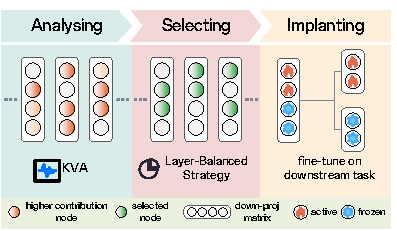
\includegraphics[width=\textwidth]{assets/pipeline.pdf}
                    \\ \scriptsize \textbf{图 1：} LoKI 三阶段微调流程。
                \end{center}
            \end{column}
            
            \begin{column}{0.5\textwidth}
                \begin{description}\setlength{\itemsep}{0.6em}
                    \item[1. 归因评分] 用\textbf{知识向量归因（KVA）}量化每个 FFN 节点对通用预训练能力的贡献度。
                    \item[2. 分层筛选] 通过\textbf{分层平衡策略}在每层等比例选出低贡献节点，维持网络层级信息流稳定。
                    \item[3. 定向植入] 冻结核心权重（$W_{\setminus S}$），仅在低贡献权重（$W_S$）上微调写入新知识。
                \end{description}
            \end{column}
        \end{columns}
    \end{frame}
    

% Slide: Stage 1 - 知识向量 Attribution (KVA)
    \begin{frame}{阶段 1：知识向量归因（KVA）}
        \begin{columns}[T]
            % --- Left Column: FFN as KV Pair ---
            \begin{column}{0.48\textwidth}
                \textbf{FFN 的键值记忆视角} \cite{geva2021}
                \begin{itemize}
                    \item \(\text{FFN}(x) = W_{down} \sigma(W_{up} x)\)
                    \item \textbf{键（$W_{up}$）：}匹配并激活输入模式。
                    \item \textbf{值（$W_{down}$）：}存储具体的语义概念与知识。
                \end{itemize}

                \begin{block}{基本分析单元：知识向量}
                    将 $W_{down}$ 的每一列 $\mathbf{v}_j$ 视为一个独立的\alert{知识向量}，对应单个中间层神经元。
                \end{block}
            \end{column}

            % --- Right Column: KVA Method ---
            \begin{column}{0.48\textwidth}
                \textbf{基于积分梯度（IG）量化节点重要性}
                \begin{itemize}
                    \item 沿激活值路径积分，计算第 $l$ 层节点 $j$ 对通用任务的贡献 \cite{sundararajan2017}：
                \end{itemize}
                \vspace{-0.2em}
                \begin{equation*}
                    \text{Attr}_{l,j}(\mathbf{x}) = \int_{\alpha=0}^{1} \frac{\partial \mathcal{L}(\alpha \cdot z_{l,j})}{\partial z_{l,j}} d\alpha
                \end{equation*}
                \vspace{-0.4em}
                \begin{alertblock}{一次性离线画像}
                    \begin{itemize}
                        \item 在 57 个学科的 \textbf{MMLU} 基准上完成通用能力探针评分 \cite{kemker2018b}。
                        \item \textbf{与任务解耦}：每个基座模型只需计算一次，可复用于任意下游任务。
                    \end{itemize}
                \end{alertblock}
            \end{column}
        \end{columns}
    \end{frame}

    % --- Stage 2: Slide 1 (Phenomenon & Heatmap) ---
    \begin{frame}{阶段 2：KVA 分数分布特征}
        \begin{columns}
            \begin{column}{0.45\textwidth}
                \begin{center}
                    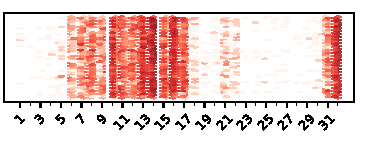
\includegraphics[width=0.92\textwidth]{assets/L3_5_H.pdf} \\
                    \vspace{0.1cm}
                    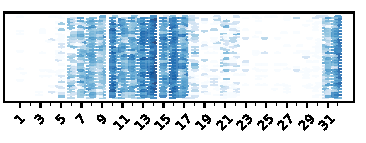
\includegraphics[width=0.92\textwidth]{assets/L3_5_L.pdf} \\
                    \vspace{0.05cm}
                    \scriptsize \textbf{图 2：} Llama 3.1-8B 的 KVA 前 5\% 节点分布热力图。
                \end{center}
            \end{column}
            \begin{column}{0.5\textwidth}
                \textbf{直接按全局排序选点会出什么问题？}
                \begin{itemize}\setlength{\itemsep}{0.4em}
                    \item \alert{层间分布极不均匀}：不同层的归因幅值差异显著 \cite{meng2023mass, dai2022b}。
                    \item \alert{同层聚集效应}：高贡献与低贡献节点往往集中在相同的活跃层中。
                    \item \alert{破坏层间路由}：若直接在全局选最低分节点，更新会过度集中在少数层，截断或覆盖后续层的信息流 \cite{hase2023}。
                \end{itemize}
            \end{column}
        \end{columns}
    \end{frame}

    % --- Stage 2: Slide 2 (Layer-Balanced Strategy Details) ---
    \begin{frame}{阶段 2：分层平衡策略}
        \textbf{设计原则：}为每一层分配相同的可训练参数配额（$q\%$），保持 Transformer 跨层计算结构的平衡 \cite{sun2025a}。
        
        \begin{block}{四步筛选流程}
            \begin{enumerate}
                \item \textbf{配额均分：}给定总预算 $T$（占比 $q\%$），每层分配固定配额 $k_l = T/L$。
                \item \textbf{单样本初筛：}对每个评测样本 $t$，在每层内选出 KVA 得分\alert{最低}的 $k_l$ 个节点。
                \item \textbf{跨样本投票：}统计每个节点在全部 $N$ 个样本中落入低贡献区间的频次 $c_{l,i}$。
                \item \textbf{确定激活集：}每层取频次最高的 $k_l$ 个节点，构成最终可训练集合 $S$。
            \end{enumerate}
        \end{block}
        
        \begin{alertblock}{结构优势}
            确保新知识均匀嵌入模型的各个处理阶段，避免局部层被过度改写。
        \end{alertblock}
    \end{frame}
    
    % Slide 7: 阶段 3：知识植入
    \begin{frame}{阶段 3：低损伤知识植入}
        对于每一层 $l$，按选定集合 $S_l$ 将 $W_{down}^{(l)}$ 拆分为两个子矩阵：
        \begin{equation*}
            W_{down}^{(l)} = [W_{S_l}; W_{\setminus S_l}] \rightarrow \begin{cases} W_{S_l} & \text{\alert{激活更新（低贡献通道）}} \\ W_{\setminus S_l} & \text{严格冻结（高贡献通道）} \end{cases}
        \end{equation*}

        \begin{block}{两种参数化模式}
            \begin{enumerate}
                \item \textbf{LoKI（直接更新）：}仅对子矩阵 $W_{S_l}$ 计算梯度并更新，零推理延迟。
                \item \textbf{LoKI-LoRA（低秩分解）：}将子矩阵更新进一步分解为低秩矩阵 $\Delta W_{S_l} = A_l B_l$ \cite{hu2022lora}，极致压缩可训练参数量。
            \end{enumerate}
        \end{block}
        \alert{工程友好：}通过矩阵重排转化为标准线性层操作，可直接接入 Llama-Factory 等主流训练框架。
    \end{frame}
    
    % Slide 8: Exp Results - Task Performance
\section{实验与分析}

    % --- Slide 1: Task 1 Downstream (ToolACE) ---
    \begin{frame}{任务 1：ToolACE 函数调用（Llama 3.1-8B）}
        \begin{table}
            \centering
            \scriptsize
            \setlength{\tabcolsep}{5pt}
            \begin{tabular}{l|c|cc|cc}
                \toprule
                \multirow{2}{*}{\textbf{方法}} & \textbf{总体} & \multicolumn{2}{c|}{\textbf{单轮准确率（$\uparrow$）}} & \textbf{多轮} & \textbf{幻觉} \\
                 & \textbf{准确率（$\uparrow$）} & 非实时 & 实时 & \textbf{准确率（$\uparrow$）} & \textbf{无关率（$\downarrow$）} \\
                \midrule
                ToolACE (LoRA)\cite{hu2022lora} & 58.32 & \textbf{87.56} & \textbf{76.10} & 7.62 & 88.05 \\
                DoRA ($r=16$) \cite{liu2024dora}& 58.90 & 82.04 & 75.61 & 16.00 & 88.92 \\
                PiSSA ($r=16$) \cite{meng2024pissa}& 53.97 & 80.56 & 72.68 & 5.62 & 92.19 \\
                \midrule
                LoKI ($q=10$) & 56.76 & 80.81 & 70.46 & 16.50 & \textbf{82.21} \\
                \textbf{LoKI ($q=20$)} & 58.16 & 81.02 & 73.26 & \alert{\textbf{17.75}} & 85.73 \\
                \textbf{LoKI ($q=30$)} & \alert{\textbf{58.93}} & 82.71 & 75.70 & 16.25 & 87.65 \\
                \textbf{LoKI-LoRA ($q=30$)} & 57.16 & 81.96 & 71.66 & 15.75 & 84.01 \\
                \bottomrule
            \end{tabular}
            \caption{Berkeley Function Calling Leaderboard V3 评测结果。}
        \end{table}
        \vspace{-0.2em}
        \begin{alertblock}{核心发现}
            \small\textbf{多轮推理翻倍提升：}LoKI ($q=20$) 多轮准确率达 \textbf{17.75\%}（官方 LoRA 仅 7.62\%）；LoKI ($q=30$) 取得最高总体准确率（\textbf{58.93\%}），并显著降低调用幻觉。
        \end{alertblock}
    \end{frame}

    % --- Slide 2: Task 1 CF (ToolACE) ---
    \begin{frame}{任务 1 遗忘评估：通用能力保留（Llama 3.1-8B）}
        \begin{table}
            \centering
            \scriptsize
            \resizebox{\textwidth}{!}{%
            \begin{tabular}{l|cccccc|c}
                \toprule
                \textbf{模型} & \textbf{TriviaQA} & \textbf{GSM8K} & \textbf{HellaSwag} & \textbf{WinoGrande} & \textbf{HumanEval} & \textbf{IF} & \textbf{平均性能损失} \\
                 &  &  &  &  &  &  & \textbf{($\downarrow$)} \\
                \midrule
                \textit{Llama 3.1-8B (基座)} & \textit{65.77} & \textit{84.46} & \textit{73.85} & \textit{62.98} & \textit{68.29} & \textit{79.76} & - \\
                \midrule
                ToolACE (LoRA) & 64.63 & 79.53 & 46.81 & 42.78 & 60.37 & 72.76 & 16.11\% \\
                DoRA ($r=16$) & 63.97 & 82.64 & 70.78 & 57.85 & 65.24 & 73.47 & 4.92\% \\
                PiSSA ($r=16$) & 52.50 & 51.40 & 37.98 & 13.18 & 15.85 & 55.95 & 48.93\% \\
                \midrule
                \textbf{LoKI ($q=10$)} & \textbf{65.85} & \textbf{84.99} & \textbf{75.14} & 61.33 & 68.90 & 77.54 & \alert{\textbf{0.34\%}} \\
                \textbf{LoKI ($q=30$)} & 65.49 & 84.61 & 71.16 & 61.09 & \textbf{70.73} & 77.94 & \alert{\textbf{1.23\%}} \\
                 \textbf{LoKI-LoRA ($q=30$)} & 64.30 & 83.47 & 70.78 & \textbf{62.51} & 70.12 & \textbf{78.21} & \alert{\textbf{1.26\%}} \\
                \bottomrule
            \end{tabular}
            }
            \caption{微调后在 6 个通用知识、推理与代码基准上的保留表现。}
        \end{table}
        \vspace{-0.2em}
        \begin{alertblock}{核心发现}
            \small\textbf{近乎零遗忘：}PiSSA 损失近半通用能力（48.93\%），LoRA 在常识推理上退化明显（16.11\%）；而 LoKI ($q=10$) 保留了基座模型 \textbf{99.66\%} 的通用能力。
        \end{alertblock}
    \end{frame}

    % --- Slide 3: Task 2 Downstream (LB Reranker) ---
    \begin{frame}{任务 2：文本重排序（Qwen 2.5-0.5B）}
        \begin{table}
            \centering
            \scriptsize
            \setlength{\tabcolsep}{6pt}
            \begin{tabular}{l|cccc}
                \toprule
                \textbf{方法} & \textbf{MAP@1} & \textbf{召回率@1} & \textbf{NDCG@1} & \textbf{精确率@1} \\
                & (\%) & (\%) & (\%) & (\%) \\
                \midrule
                DoRA ($r=8$) \cite{liu2024dora}& -8.7 & -8.7 & -11.2 & -10.4 \\
                PiSSA ($r=8$) \cite{meng2024pissa}& -9.6 & -9.6 & -9.7 & -10.2 \\
                CorDA ($r=8$) \cite{yang2024corda}& -3.3 & -3.1 & -2.6 & -3.3 \\
                \midrule
                LoKI ($q=5$) & -3.1 & -3.1 & -2.2 & -1.8 \\
                LoKI ($q=10$) & -2.3 & -2.3 & -0.3 & -0.5 \\
                \textbf{LoKI ($q=30$)} & \alert{\textbf{+1.0}} & \alert{\textbf{+1.0}} & \alert{\textbf{+2.1}} & \alert{\textbf{+2.5}} \\
                \bottomrule
            \end{tabular}
            \caption{BEIR 基准上相对于全参数微调的性能差异（正值代表超越全量微调）。}
        \end{table}
        \vspace{-0.2em}
        \begin{alertblock}{核心发现}
            \small\textbf{以 30\% 参数超越全量微调：}常规 PEFT 方法在小模型重排序上普遍落后于全量微调，而 LoKI ($q=30$) 在全部核心检索指标上实现反超。
        \end{alertblock}
    \end{frame}

    % --- Slide 4: Task 2 CF (LB Reranker) ---
    \begin{frame}{任务 2 遗忘评估：避免小模型崩溃（Qwen 2.5-0.5B）}
        \begin{table}
            \centering
            \scriptsize
            \setlength{\tabcolsep}{2.5pt}
            \resizebox{\textwidth}{!}{%
            \begin{tabular}{l|cccccc|c}
                \toprule
                \textbf{模型} & \textbf{TriviaQA} & \textbf{GSM8K} & \textbf{HellaSwag} & \textbf{WinoGrande} & \textbf{HumanEval} & \textbf{IF} & \textbf{平均性能损失} \\
                 &  &  &  &  &  &  & \textbf{($\downarrow$)} \\
                \midrule
                \textit{Qwen 2.5-0.5B (基座)} & \textit{24.37} & \textit{39.65} & \textit{30.98} & \textit{44.20} & \textit{26.83} & \textit{33.39} & - \\
                \midrule
                全参数微调 & 4.65 & 2.65 & \alert{0.00} & \alert{0.00} & \alert{0.00} & 23.20 & 84.13\% \\
                DoRA ($r=8$) & 19.30 & 34.01 & 22.21 & 44.70 & 25.22 & 31.67 & 12.23\% \\
                CorDA ($r=8$) & 4.64 & 2.43 & \alert{0.00} & \alert{0.00} & \alert{0.00} & 23.20 & 84.22\% \\
                \midrule
                \textbf{LoKI ($q=30$)} & 20.10 & \textbf{37.60} & \textbf{38.39} & \textbf{43.96} & \textbf{26.83} & 32.25 & \alert{\textbf{0.46\%}} \\
                \bottomrule
            \end{tabular}
            }
            \caption{0.5B 小模型微调后在 6 个通用基准上的保留表现。}
        \end{table}
        \vspace{-0.2em}
        \begin{alertblock}{核心发现}
            \small\textbf{防止小模型崩溃：}0.5B 模型冗余度低，全量微调与 CorDA 在代码和常识基准上直接归零（损失超 84\%）；LoKI 保护核心参数，损失仅 \textbf{0.46\%}。
        \end{alertblock}
    \end{frame}
    
    % Slide 10: Ablation Study
    \begin{frame}{消融实验：KVA 定位与分层策略缺一不可}
        \begin{columns}[T]
            % --- Column 1: Validation of KVA ---
            \begin{column}{0.49\textwidth}
                \begin{block}{1. 验证 KVA：高分节点是否真关键？}
                    将每层 $1\%$ 的高贡献节点（S-H）或低贡献节点（S-L）置零：
                    \vspace{0.2cm}
                    
                    \centering
                    \small
                    \begin{tabular}{l|c}
                        \toprule
                        \textbf{置零策略（$q=1$）} & \textbf{通用性能跌幅 $\downarrow$} \\
                        \midrule
                        \textbf{S-H} (置零高贡献) & \alert{\textbf{36.73\%}} \\
                        S-L (置零低贡献) & \textcolor{blue}{\textbf{11.35\%}} \\
                        \midrule
                        \textit{破坏力差距} & \textit{$\approx$ \textbf{3.2 倍}} \\
                        \bottomrule
                    \end{tabular}
                \end{block}
                \vspace{0.1cm}
                \footnotesize \textbf{结论：}KVA 准确定位了核心知识通道，高分节点的破坏力是低分节点的 3.2 倍。
            \end{column}

            % --- Column 2: Validation of Strategy ---
            \begin{column}{0.49\textwidth}
                \begin{block}{2. 验证分层平衡：为何不能全局直接选？}
                    对比全局选最高（G-H）、全局选最低（G-L）与分层均衡选最低（LoKI）：
                    \vspace{0.2cm}
                    
                    \centering
                    \small
                    \begin{tabular}{l|c}
                        \toprule
                        \textbf{选点策略（$q=10$）} & \textbf{通用性能跌幅 $\downarrow$} \\
                        \midrule
                        全局高值 (G-H) & 39.04\% \\
                        全局低值 (G-L) & 30.48\% \\
                        \midrule
                        \textbf{分层平衡 (LoKI)} & \textcolor{green!60!black}{\textbf{8.86\%}} \\
                        \bottomrule
                    \end{tabular}
                \end{block}
                \vspace{0.1cm}
                \footnotesize \textbf{结论：}全局选点会掏空特定层并导致严重退化（30.48\%），分层均衡将损伤降至 8.86\%。
            \end{column}
        \end{columns}
    \end{frame}
    
    % Slide 11: 结论
    \section{结论}
    \begin{frame}{总结}
        \begin{block}{核心工作}
            \begin{itemize}\setlength{\itemsep}{0.4em}
                \item \textbf{机制引导微调（LoKI）：}锁定关键记忆、重用冗余参数，从根源上缓解微调带来的灾难性遗忘。
                \item \textbf{知识向量归因（KVA）：}利用积分梯度对模型做一次性通用能力画像，精准区分高低贡献节点。
                \item \textbf{分层平衡策略：}按层均匀分配更新配额，维持 Transformer 跨层信息流稳定。
                \item \textbf{卓越的实证表现：}在 8B 与 0.5B 模型上均实现强下游性能与近乎零遗忘（$<1.3\%$ 损失）兼得。
            \end{itemize}
        \end{block}

        \vspace{0.3cm}
        \begin{center}
            \alert{\textbf{打通可解释性机理分析与高效微调落地。}}
        \end{center}
    \end{frame}
    
    % Q&A Page with Logos and QR Codes
    \section{问答}
\begin{frame}{感谢聆听！}
    \begin{center}
        \begin{tabular}{ccc}
            
\includegraphics[height=1cm]{assets/arxiv-logo-1.png} & 
            
\includegraphics[height=1cm]{assets/GitHub-Logo-700x394.png} & 
            
\includegraphics[height=1cm]{assets/WeChat.png} \\[0.5cm]
            
            
\includegraphics[width=3cm]{assets/arxiv_code.png} & 
            
\includegraphics[width=3cm]{assets/github_code.png} & 
            
\includegraphics[width=3cm]{assets/wechat_code.png} \\[0.2cm]
            
            \small arXiv:2505.22120 & 
            \small github.com/Nexround/LoKI & 
            \small 联系我们 \\
        \end{tabular}
    \end{center}
\end{frame}

    % 参考文献 Section
    \section{参考文献}
    \begin{frame}[shrink=15]{参考文献}
        \tiny
        \setlength{\itemsep}{0pt}
        \setlength{\parskip}{0pt}
        \begin{thebibliography}{99}
        \setlength{\itemsep}{1pt}
        
        \bibitem{brown2020}
        Brown, T. et al. (2020). Language Models are Few-Shot Learners. \textit{NeurIPS}.
        \bibitem{cohen2023}
        Cohen, R. et al. (2023). Crawling The Internal Knowledge-Base of Language Models. \textit{EACL}.
        \bibitem{dai2022b}
        Dai, D. et al. (2022b). Knowledge Neurons in Pretrained Transformers. \textit{ACL}.
        \bibitem{geva2021}
        Geva, M. et al. (2021). Transformer Feed-Forward Layers Are Key-Value Memories. \textit{EMNLP}.
        \bibitem{hase2023}
        Hase, P. et al. (2023). Does Localization Inform Editing? \textit{NeurIPS}.
        \bibitem{hu2022lora}
        Hu, E. J. et al. (2022). LoRA: Low-rank adaptation of large language models. \textit{ICLR}.
        \bibitem{kemker2018b}
        Kemker, R. et al. (2018b). Measuring Catastrophic Forgetting in Neural Networks. \textit{AAAI}.
        \bibitem{kotha2024}
        Kotha, S. et al. (2024). Understanding CF in LMs via Implicit Inference. \textit{ICLR}.
        \bibitem{li2024revisiting}
        Li, H. et al. (2024). Revisiting Catastrophic Forgetting in Large Language Model Tuning. \textit{EMNLP}.
        \bibitem{liu2024dora}
        Liu, S. et al. (2024). DoRA: Weight-Decomposed Low-Rank Adaptation. \textit{ICML}.
        \bibitem{liu2024toolace}
        Liu, W. et al. (2024). ToolACE: Winning the Points of LLM Function Calling. \textit{arXiv}.
        \bibitem{luo2025}
        Luo, Y. et al. (2025). An Empirical Study of CF in LLMs During Continual Fine-tuning. \textit{arXiv}.
        \bibitem{meng2022locating}
        Meng, K. et al. (2022). Locating and Editing Factual Associations in GPT. \textit{NeurIPS}.
        \bibitem{meng2023mass}
        Meng, K. et al. (2023a). Mass-Editing Memory in a Transformer. \textit{ICLR}.
        \bibitem{meng2024pissa}
        Meng, F. et al. (2024). PiSSA: Principal Singular Values and Singular Vectors Adaptation. \textit{NeurIPS}.
        \bibitem{petroni2019}
        Petroni, F. et al. (2019). Language Models as Knowledge Bases? \textit{EMNLP}.
        \bibitem{qwen2025}
        Qwen et al. (2025). Qwen2.5 Technical Report. \textit{arXiv}.
        \bibitem{radford2018}
        Radford, A. \& Narasimhan, K. (2018). Improving Language Understanding by Generative Pre-Training.
        \bibitem{sanh2020}
        Sanh, V. et al. (2020). Movement Pruning: Adaptive Sparsity by Fine-Tuning. \textit{NeurIPS}.
        \bibitem{sun2025a}
        Sun, Q. et al. (2025a). Transformer Layers as Painters. \textit{AAAI}.
        \bibitem{sundararajan2017}
        Sundararajan, M. et al. (2017). Axiomatic Attribution for Deep Networks. \textit{ICML}.
        \bibitem{yang2024corda}
        Yang, Y. et al. (2024). CorDA: Context-Oriented Decomposition Adaptation. \textit{NeurIPS}.

        \end{thebibliography}
    \end{frame}
    
\end{document}
